% (approx. 500-800 words)

\section{Evaluation}
\label{sec:eval}
The purpose of this section is to explain and show the obtained results across different runs. In particular, it is worth mentioning that
lots of default valued hyper-parameters have been used such as:
\begin{itemize}
    \item \textit{batch size}, for both the training of the BiSTM (\Cref{subsec:subj}) and the final polarity evaluation procedure, of $128$
        samples. In the case of the binary classifier (~\cite{sequence}), a batch size of $64$ has been used;
    \item concerning the \textit{dataset split} dimensions:
        \begin{itemize}
            \item the subjectivity dataset into training set ($80\%$) and test set ($20\%$). The training set has been further splitted 
            considering a randomly sampled $10\%$ for evaluation pruposes;
            \item the IMDB dataset has been splitted following the built-in splitting format of the dataset itself ($25K$ samples for training
            and $25K$ sampels for evaluation)
        \end{itemize}
    \item during the training procedure an \textit{early stopper} has been used to implement an early stopping techinque. To do so, the 
        difference between the accuracy at the previous run and the current one is investiagate. If the latter is grater than $MIN\_DELTA=0.075$, 
        then the training procedure is interrupted and the last model saved;
    \item the BiLSTM model has been trained for $10$ \textit{epochs} and the binary classifier just for one (for time reasons);
    \item regarding the BiLSTM model, the multiple runs have been performed using a randomly selected seeds: $[91, 11, 57, 822, 19]$;
    \item for the AdamW and Adam optimiers, the learning rates used are $0.001$ and $0.0002$ respectively. 
\end{itemize}


\subsection{Evaluation metric}
\label{subsec:metric}
Across the different models, several evaluation metrics have been used. 
\subsubsection{Baseline}
Concerning the baseline, a simple \texttt{accuracy} metric has been used across a 10-fold cross validation procedure.
\subsubsection{Custom model}
As regards my proposed model, different evaluation metrics have been used for the different components:
\begin{itemize}
    \item for the BiLSTM model, as well as for the final evaluation on the polarity dataset, to detect subjectivity labels, a simple cumulative accuracy metric, defined as the sum of all the agreeements
    across all the batches over the number of samples in the training set, has been used;
    \item for the \textit{BertForSequenceClassification} instance an ensamble of metrics has been computed, exploiting the 
    \texttt{accuracy\_score} and \texttt{precision\_recall\_fscore\_support} methods provided by the \texttt{sklearn} python module. 
    In particular, the function used to compute these metrics can be analysed in \textbf{\Cref{alg:binaryclf}}
    \item as for the BiLSTM model, also for the final polarity classification step a cumulative accuracy has been used, where the agreeements
    between the predictions given by the pre-fine-tuned binary classifier and the ground truth are investigated and quantified.
\end{itemize}


\begin{algorithm}
    \SetAlgoLined
    \DontPrintSemicolon
    \KwIn{pred}    
    \KwOut{accuracy, f1, precision, recall}
    \CommentSty{\color{blue}}
    precision, recall, f1, \_  $\gets$ precision\_recall\_fscore\_support(labels, preds, average='binary')\;
    acc $\gets$ accuracy\_score(labels, preds)\;

    return\{\;
            \hspace{5mm}'accuracy': acc,\;
            \hspace{5mm}'f1': f1,\;
            \hspace{5mm}'precision': precision,\;
            \hspace{5mm}'recall': recall\;
        \}

\caption{Metric computation function for Trainer interface.}
\label{alg:binaryclf}

\end{algorithm}

Of course, the overall objective is to maximise the accuracy on both subjectivity and polarity datasets by minimizing the losses used during 
the training procedure as application of the maximisation of the posterior probabilities.

\subsection{Results}
\label{subsec:res}
In this particular section, the results obtained across different runs and experiments are analysised as much in detail as possible.\\
\begin{figure}
    \centering
    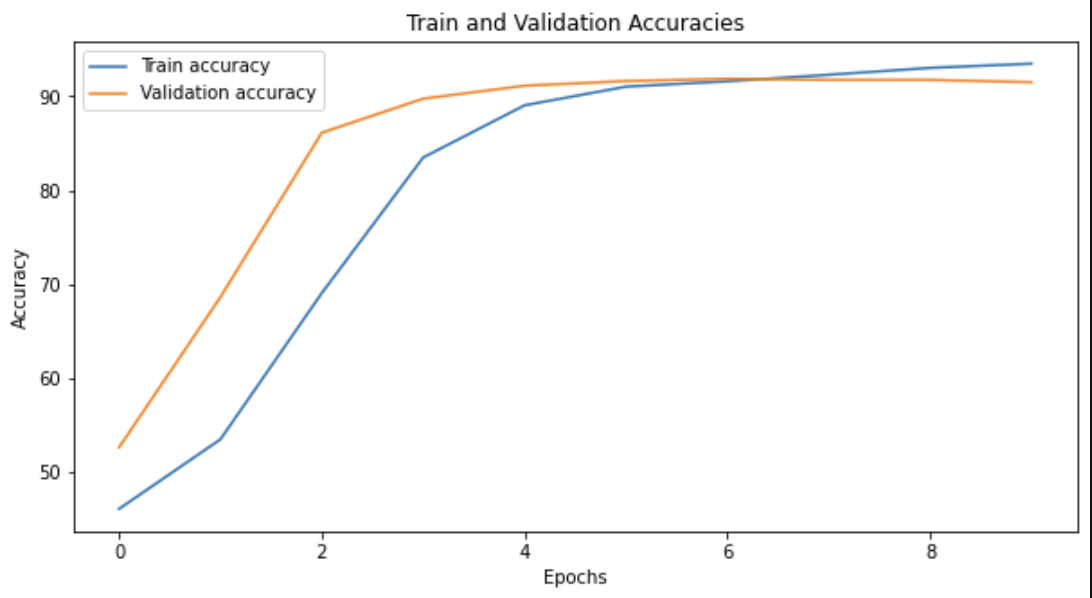
\includegraphics[scale=0.28]{Images/singlerunacc.png}
    \vspace{-1.0em}
    \caption{BiLSTM model training and evaluation accuracies on a single run.}
    \vspace{-1.0em}
    \label{fig:singlerunacc}
\end{figure}

\begin{figure}
    \centering
    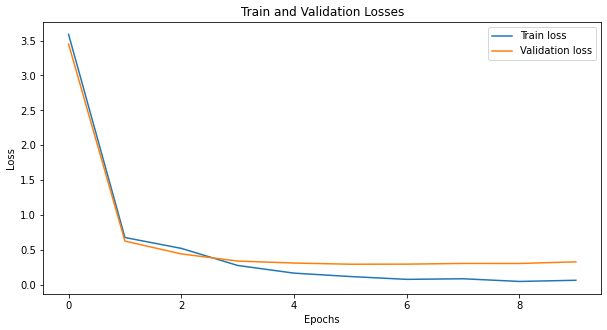
\includegraphics[scale=0.28]{Images/singlerunloss.png}
    \vspace{-1.0em}
    \caption{BiLSTM model training and evaluation losses on a single run.}
    \vspace{-1.0em}
    \label{fig:singlerunloss}
\end{figure}


In \textbf{\Cref{fig:singlerunacc}} and \textbf{\Cref{fig:singlerunloss}} it is possible to respectively appreciate the training and 
evaluation accuracies and losses, on a single run for the BiLSTM model (discussed in \Cref{subsec:cutsom}. \\
Since a single run is not very expressive and fully reliable, I decided to perform a 5-fold cross validation addressing both the average 
accuracy as well as the variance across the different runs (for details refer to )


\begin{center}
    \begin{threeparttable}
    \caption{5-fold cross validation polarity results}
        \begin{tabular}{cccccccc}
            \hline
            \thead{Seeds} & \thead{91} & \thead{11} & \thead{57} & \thead{822} & \thead{19} & \thead{Avg} & \thead{Var}\\
            \hline
            Accuracy & $89.5$ & $90.8$ & $91.05$ & $90.25$ & $89.1$ & $90.14$ & $0.74$\\
            \hline
        \end{tabular}
        \label{tab:ks}
    \end{threeparttable}
\end{center}
